% How an abliterated model is actually produced, end to end.
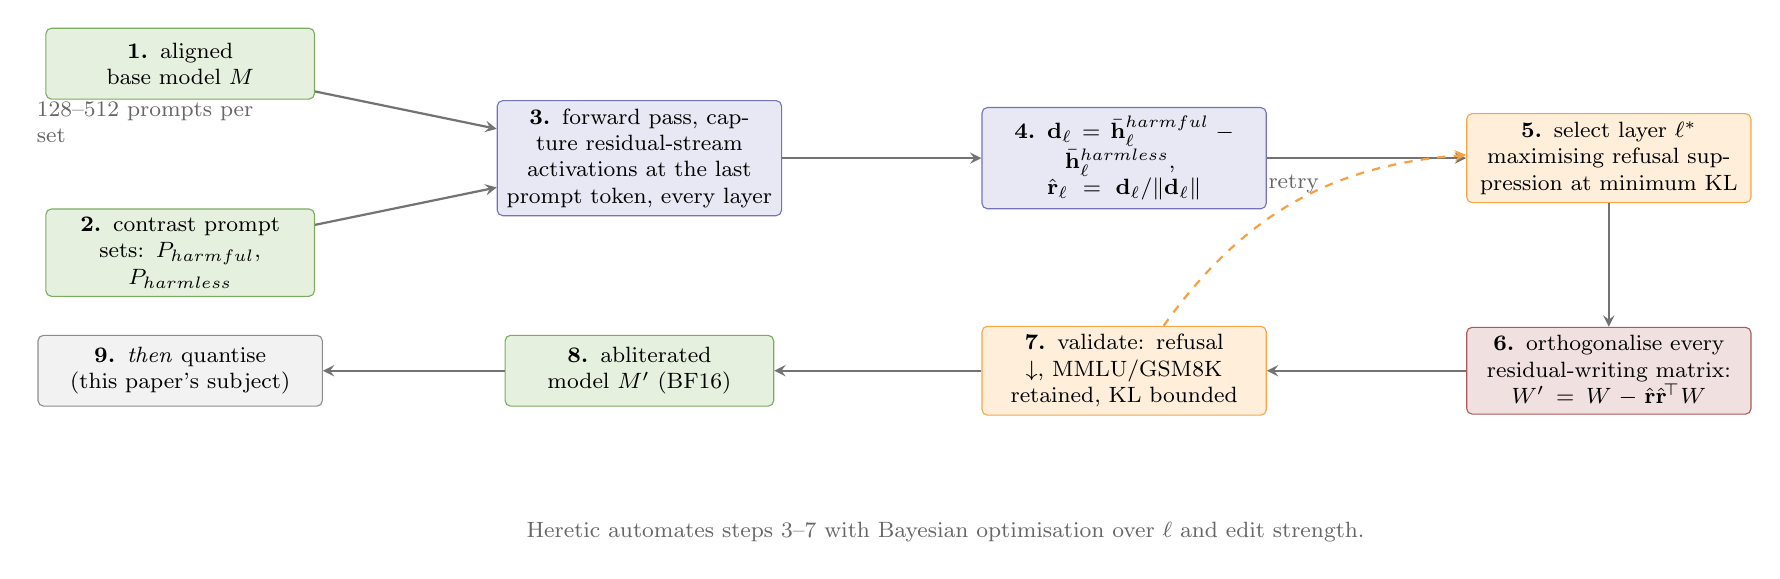
\begin{tikzpicture}[
  font=\footnotesize, x=1.62mm, y=1.5mm, >=stealth,
  stp/.style={draw=NavyBlue!55, fill=NavyBlue!9, rounded corners=2pt,
               text width=34mm, align=center, inner sep=3pt, minimum height=9mm},
  data/.style={draw=OliveGreen!60, fill=OliveGreen!10, rounded corners=2pt,
               text width=32mm, align=center, inner sep=3pt, minimum height=9mm},
  edit/.style={draw=Maroon!65, fill=Maroon!12, rounded corners=2pt,
               text width=34mm, align=center, inner sep=3pt, minimum height=9mm},
  gate/.style={draw=BurntOrange!70, fill=BurntOrange!12, rounded corners=2pt,
               text width=34mm, align=center, inner sep=3pt, minimum height=9mm},
  ar/.style={->, black!55, thick},
  n/.style={font=\footnotesize, text=black!60},
]
\node[data]  (m0) at (0,26)   {\textbf{1.} aligned base model $M$};
\node[data]  (ps) at (0,10)   {\textbf{2.} contrast prompt sets: $P_{\text{harmful}}$, $P_{\text{harmless}}$};
\node[stp]  (act) at (36,18) {\textbf{3.} forward pass, capture residual-stream activations at the last prompt token, every layer};
\node[stp]  (dir) at (74,18) {\textbf{4.} $\mathbf{d}_\ell = \bar{\mathbf h}^{\text{harmful}}_\ell - \bar{\mathbf h}^{\text{harmless}}_\ell$, \; $\hat{\mathbf r}_\ell = \mathbf{d}_\ell/\|\mathbf{d}_\ell\|$};
\node[gate]  (sel) at (112,18){\textbf{5.} select layer $\ell^\ast$ maximising refusal suppression at minimum KL};
\node[edit]  (ed) at (112,0)  {\textbf{6.} orthogonalise every residual-writing matrix: $W'=W-\hat{\mathbf r}\hat{\mathbf r}^{\!\top}W$};
\node[gate]  (val) at (74,0)  {\textbf{7.} validate: refusal $\downarrow$, MMLU/GSM8K retained, KL bounded};
\node[data]  (out) at (36,0)  {\textbf{8.} abliterated model $M'$ (BF16)};
\node[stp, fill=black!5, draw=black!45] (q) at (0,0)
  {\textbf{9.} \emph{then} quantise \\ (this paper's subject)};

\draw[ar] (m0) -- (act); \draw[ar] (ps) -- (act);
\draw[ar] (act) -- (dir); \draw[ar] (dir) -- (sel); \draw[ar] (sel) -- (ed);
\draw[ar] (ed) -- (val); \draw[ar] (val) -- (out); \draw[ar] (out) -- (q);
\draw[ar, BurntOrange!75, dashed] (val) to[bend left=25] node[n, above] {retry} (sel);

\node[n, anchor=west, text width=30mm] at (-12,21) {128--512 prompts per set};
\node[n, anchor=north, text width=150mm, align=center] at (60,-12)
  {Heretic automates steps 3--7 with Bayesian optimisation over $\ell$ and edit strength.};
\end{tikzpicture}
